\chapter{Thuật toán Vegas}\label{ch:3}
\section{Giới thiệu}\label{sec:3.1}
Phương pháp Monte Carlo sử dụng các thuật toán để giải quyết các bài toán trên máy tính bằng cách lấy mẫu ngẫu nhiên. Kết quả của phương pháp Monte Carlo này càng chính xác khi số lượng mẫu càng tăng. Theo quy luật số lớn khi kích thước mẫu càng lớn thì tốc độ hội tụ của tích phân càng lớn, nhưng khi mở rộng số chiều của tích phân thì số lượng mẫu cũng phải tăng theo. Điều này cũng làm ảnh hưởng đến tốc độ tính toán của máy tính. Nếu cố định số lượng mẫu thì tốc độ hội tụ của tích phân sẽ giảm khi số chiều tăng lên. Nhìn chung, tốc độ hội tụ của phương pháp Monte Carlo là khá thấp.Vì vậy, phương pháp tích phân Monte-Carlo sử dụng thuật toán Vegas \cite{vegas} sẽ giải quyết hiệu quả với các tích phân nhiều chiều.
\par
Đặc điểm thuật toán: 
\begin{enumerate}
      \item Phương sai của tích phân thì được tính toán dễ dàng.
      \item Hàm tính tích phân không cần liên tục và các hàm bước nhảy cũng không gặp khó khăn trong tính toán khi sử dụng thuật toán mới. Vì thế để tính tích phân nhiều chiều là việc đơn giản.
      \item Tốc độ hội tụ không phụ thuộc vào số chiều của tích phân.
      \item Đây là thuật toán thích nghi, nó tự động tập trung tính toán tích phân tại những vùng có tích phân quan trọng nhất.
\end{enumerate}
Đặc điểm (1) và (3) là phổ biến trong tất cả phương pháp Monte Carlo. Với (4) là một tính năng quan trọng nhất trong thuật toán này. Vấn đề chính trong tính toán các tích phân nhiều chiều là việc tăng số lượng mẫu theo cấp số nhân khi tăng số chiều. 
Do đó, mục đích chung của thuật toán để tính toán tích phân nhiều chiều là thích nghi sau mỗi vòng lặp.
\section{Tích phân Monte Carlo sử dụng thuật toán Vegas}\label{sec:3.2}
Monte Carlo là phương pháp sử dụng số ngẫu nhiên để tính toán, vì vậy để có ước tính tích phân chính xác thì 
vấn đề giảm phương sai cần được quan tâm. 
Để giảm phương sai, tất cả những gì có thể làm là tăng số lượng mẫu M. 
Muốn giảm phương sai xuống hai lần thì phải tăng gấp bốn lần số mẫu. 
Đối với các hàm tích phân nhiều chiều, 
số lượng mẫu tăng theo cấp số nhân khi số chiều tăng lên. 
Do đó, có nhiều phương pháp đã được nghiên cứu để giảm phương sai mà không cần tăng số lượng mẫu M. 
Như vậy, phương pháp lấy mẫu trọng và phương pháp lấy mẫu phân tầng được sử dụng trong thuật toán Vegas để giảm phương sai.
\par
\subsection{Lấy mẫu trọng}\label{subsec:3.2.1}
Lấy mẫu trọng là phương pháp làm giảm phương sai bằng cách chọn hàm mật độ xác suất bất kỳ. 
Nhưng nếu chọn hàm mật độ xác suất tương tự với hình dạng của hàm f(x) thì kết quả tích phân càng chính xác. 
Tuy nhiên, nếu đặt nhiều mẫu tại những nơi mà tích phân có đóng góp lớn, thì phương sai của tích phân Monte Carlo giảm đáng kể. 
Ở đây hàm mật độ $p(x)$ được thay đổi để giảm phương sai. Như đã biết, phương sai được tối ưu khi: 
\begin{align}
      p(x)=\frac{|f(x)|}{\int_\Omega{dx|f(x)|}}\label{ctmauqt}
  \end{align}
Do đó, khi sử dụng gieo điểm trọng tích phân sẽ được tính tập trung tại nơi tích phân có độ lớn lớn nhất.\par
\subsection{Lấy mẫu phân tầng}\label{subsec:3.2.2}
Để giảm phương sai, thể tích tích phân có thể được chia thành $N$ khối thể tích nhỏ với các kích thước khác nhau. 
Sau đó tích phân Monte Carlo được thực hiên trong mỗi khối thể tích nhỏ. 
Với mỗi khối thể tích nhỏ này sử dụng $M/N$ điểm ngẫu nhiên. 
Khi kích thước của khối thể tích nhỏ bị thay đổi thì phương sai sẽ được tính toán lại và được tối ưu khi phương sai của mỗi khối thể tích nhỏ này là như nhau (=$\sigma^2/N$). 
Do đó, khi sử dụng gieo điểm phân tầng, tích phân sẽ được tập trung tại nơi có sai số lớn nhất, 
tức là nơi tích phân vừa lớn và vừa dao động mạnh.\\
Bước đầu tiên trong thuật toán sử dụng phương pháp lấy mẫu phân tầng, là chia siêu khối thể tích của tích phân $n$ chiều thành $N^n$ siêu khối nhỏ như nhau. 
Bằng cách sử dụng một lưới hình chữ nhật đồng nhất. 
Mỗi siêu khối nhỏ sử dụng hai điểm để đóng góp vào việc tính tích phân Monte Carlo và phương sai. 
Các phương sai từ các siêu khối nhỏ sau đó được sử dụng để định nghĩa lại không gian lưới mới dọc theo mỗi trục 
và không gian lưới mới này sẽ được sử dụng cho lần lặp tiếp theo. 
Và phải giữ cho tổng số khối nhỏ không đổi. 
Do vậy qua mỗi vòng lặp thì các khối nhỏ có thể tập trung dần về nơi có phương sai lớn nhất trước đó, 
như vậy phương sai được giảm.\\
Thuật toán lấy mẫu phân tầng được sử dụng rộng rãi trong ngành Vật lý Lý thuyết và rất thành công cho nhiều ứng dụng tính toán hai chiều trở lên. 
Ưu điểm lớn nhất của phương pháp là khả năng thích nghi của tích phân đang được tính toán. 
Tuy nhiên khả năng thích nghi của nó được quyết định bởi số lượng đoạn được chia dọc theo mỗi trục $N$,
và $N$ bị giới hạn bởi tổng số tích phân $M$ được cho phép ở mỗi vòng lặp.
\begin{align}
      M=2N^n
  \end{align}
Hạn chế này cho thấy một khuyết điểm khi số chiều lớn.
\subsection{Thuật toán Vegas}\label{subsec:3.2.3}
Hạn chế từ phương pháp lấy mẫu phân tầng có thể tránh được bằng cách sử dụng phương pháp lấy mẫu trọng để giảm phương sai. 
Phương pháp lấy mẫu trọng dường như cho thấy kém hiệu quả hơn phương pháp lấy mẫu phân tầng. 
Tuy nhiên, khả năng thích nghi của phương pháp vượt trội hơn khi được thể hiện ở bài toàn có số chiều lớn. 
Vì vậy thuật toán Veags sẽ kết hợp cả hai phương pháp trên để xử lý bài toán.\par
Xét tích phân của một biến $\textbf{x}(x1,...,xn)$ trên không gian mẫu $\Omega$.
\begin{align}
      I=\int_\Omega{dxf(x)}
  \end{align}
  Chon ngẫu nhiên M biến \textbf{x} từ một phân bố trong không gian mẫu $\Omega$ với xác suất $p(x)$. Cho thấy được tích phân xấp xĩ bằng
  \begin{align}
      S^{(1)}={\frac{1}{M}}{\sum_\textbf{x}{\frac{f(\textbf{x})}{p(\textbf{x})}}}\label{pt3.4}
  \end{align}
Trong đó hàm mật độ xác suất được chuẩn hóa thành
\begin{align}
      \int_{\Omega}{d\textbf{x}p(\textbf{x})}=1
\end{align}
Đại lượng $S^{(1)}$ được kì vọng sẽ dao động về giá trị đúng của tích phân. Tương ứng với mỗi tập hợp các điểm $M$ ngẫu nhiên là 1 đại lượng ngẫu nhiên $S^{(1)}$ khác nhau. 
Phương sai của dao động này là:
\begin{align}
      \sigma^2=\left\{\int_{\Omega}d\textbf{x}\frac{f^2(\textbf{x})}{p(\textbf{x})}-\left[\int_{\Omega}d\textbf{x}f(\textbf{x})\right]^2\right\}M^{-1}\label{pt3.7}
\end{align}
Đối với tập hợp điểm M lớn thì phương sai là
\begin{align}
      \sigma^2\cong\frac{S^{(2)}-S^{(1)}}{M-1}\label{pt3.7}
\end{align}
tại: 
\begin{align}
      S^{(2)}=\frac{1}{M}{\sum_\textbf{x}}\left(\frac{f(\textbf{x})}{p(\textbf{x})}\right)^2
\end{align}
\textbf{Xem xét tích phân một chiều }\\
\begin{align}
      I=\int_0^1{dxf(x)}
\end{align}
Khởi tạo $M$ điểm với mật độ xác suất đều. Ngoài việc ước tính giá trị tích phân $ \ref{pt3.4} $ và phương sai $ \ref{pt3.7} $, các điểm M dùng để tính tích phân cũng có thể được sử dụng 
để tính toán lại mật độ xác suất tốt hơn cho vòng lặp tiếp theo. 
Trong phương pháp này phương sai sẽ được giảm dần qua các vòng lặp.\par
Có một số kỹ thuật để tạo ra dãy số giả ngẫu nhiên với phân bố đều. 
Tuy nhiên, khó khăn hơn khi muốn tạo ra dãy số ngẫu nhiên với một phân bố bất kỳ có mật độ $p(x)$. 
Trong bài toán hiện tại sẽ đơn giản hơn nếu ta coi $p(x)$ là một hàm bước nhảy với $N$bước. 
Xác suất của một số ngẫu nhiên được chọn từ một bước nhảy bất kỳ thì được xác định là một hằng số $1/N$ cho tất cả các bước ($0=x_0 < … X_N =1, {\Delta}x_i = x_i-x_{i-1}$).
\begin{align}
      p(x)=\frac{1}{N{\Delta}x_i}
\end{align}
trong đó $x_i-{\Delta}x_i\leq x \leq x_i$, $i=1, ...,N $ 
Phân phối xác suất được điều chỉnh theo các tích phân từng phần cụ thể bằng cách thay đổi kích thước của các đoạn ${\Delta}x_i$. Nếu $N$ bị giới hạn bởi bộ nhớ máy tính  thì $N$ là một hằng số ($N = 50 $đến $100$).
Cho các $M$ điểm để tính tích phân và mật độ xác suất, kích thước các đoạn ${\Delta}x_i$ được điều chỉnh lại bằng cách chia nhỏ mỗi đoạn thành$ m_i + 1$ đoạn nhỏ hơn, tại
\begin{align}
      m_i=K\left\{ \left[ \frac{\overline{f_i}{\Delta}x_i}{\sum_j{f_j{\Delta}x_j}}-1\right]{\frac{1}{log\left[ {\frac{\overline{f_i}{\Delta}x_i}{\sum_j\overline{f_j}{\Delta}x_j}}\right]}}\right\}\label{ptmi}
\end{align}
với
\begin{align}
      \overline{f_i} \equiv {\sum_{x\in{x_i-\Delta}x_i}^{x_i}}{f(x)}\label{pt3.12}
\end{align}
Toàn miền lấy tích phân sẽ bị chia nhỏ thành $k+1$ đoạn con ($k=1000$). \label{giaithichmi}
Số lượng đoạn con trong mỗi đoạn được xác định trong biểu thức $ \ref{ptmi} $,
mỗi đoạn con của mỗi đoạn ${\Delta}x_i $ là như nhau. Sự đóng góp của mỗi đoạn cho hàm trọng sẽ tăng tỉ lệ với sự đóng góp của nó cho tích phân $|f(x)|$, 
như yêu cầu trong phương trình $ \ref{ctmauqt}$. Vì tổng số đoạn ${\Delta}x_i $ phải giữ nguyên bằng N, 
các đoạn con sẽ được gom lại thành các đoạn ${\Delta}x_i $ mới sao cho số đoạn con trong mỗi đoạn ${\Delta}x_i $ là như nhau. 
Kết quả, kích thước của các đoạn ${\Delta}x_i $ được thay đổi nhưng tổng số đoạn ${\Delta}x_i $ không đổi. Vì vậy, đoạn ${\Delta}x_i $ có kích thước nhỏ nhất là nơi $|f(x)|$ lớn nhất. 
Lưới mới này sẽ được dùng và sẽ được điều chỉnh trong mỗi lần lặp cho tới khi lưới đạt tối ưu (tức $m_i=m_j$,i,j=1,…,N ). 
Mỗi tích phân và sai số được sử dụng để tính toán cho tổng tích phân.\par
Các giá trị ước tính của tích phân và phương sai của vòng lặp sẽ được sử dụng cho phần tính toán tích phân cuối cùng sau các vòng lặp. 
\begin{align}
      I=\sigma_I^2\sum_{i=1}^{m}{\frac{I_i}{{\sigma_i}^2}}
\end{align}
\begin{align}
      \sigma=\left(\sum_{i=1}^{m}{\frac{1}{{\sigma_i}^2}}\right)^{1/2}
\end{align}
\textbf{Xem xét tích phân n chiều}\\
Thuật toán mô tả bên dưới được tổng quát hóa với mục đích xử lý tích phân nhiều chiều. Minh họa cho sự thay đổi 
\begin{align}
      \int_{0}^{1}{dx} \int_{0}^{1}{dyf(x,y)} 
\end{align}
Lúc này, hàm mật độ xác suất được viết lại như sau: 
\begin{align}
      p(x,y)=p_x(x)p_y(y)
\end{align}
Do đó thuật toán một chiều có thể áp dụng dọc theo mỗi trục. Phương trình $ \ref{pt3.12} $ được viết lại
\begin{align}
      \overline{f_i} \equiv {\sum_{x\in{x_i-\Delta}x_i}^{x_i}}{\sum_y{\frac{f^2(x,y)}{P_y^2(y)}}}
\end{align}
\newline
\newline
\newline
Hình $ \ref{hinh3.1} $ mô tả lại các bước thực hiện của thuật toán Vegas.
\begin{figure}[H]
      \centering
      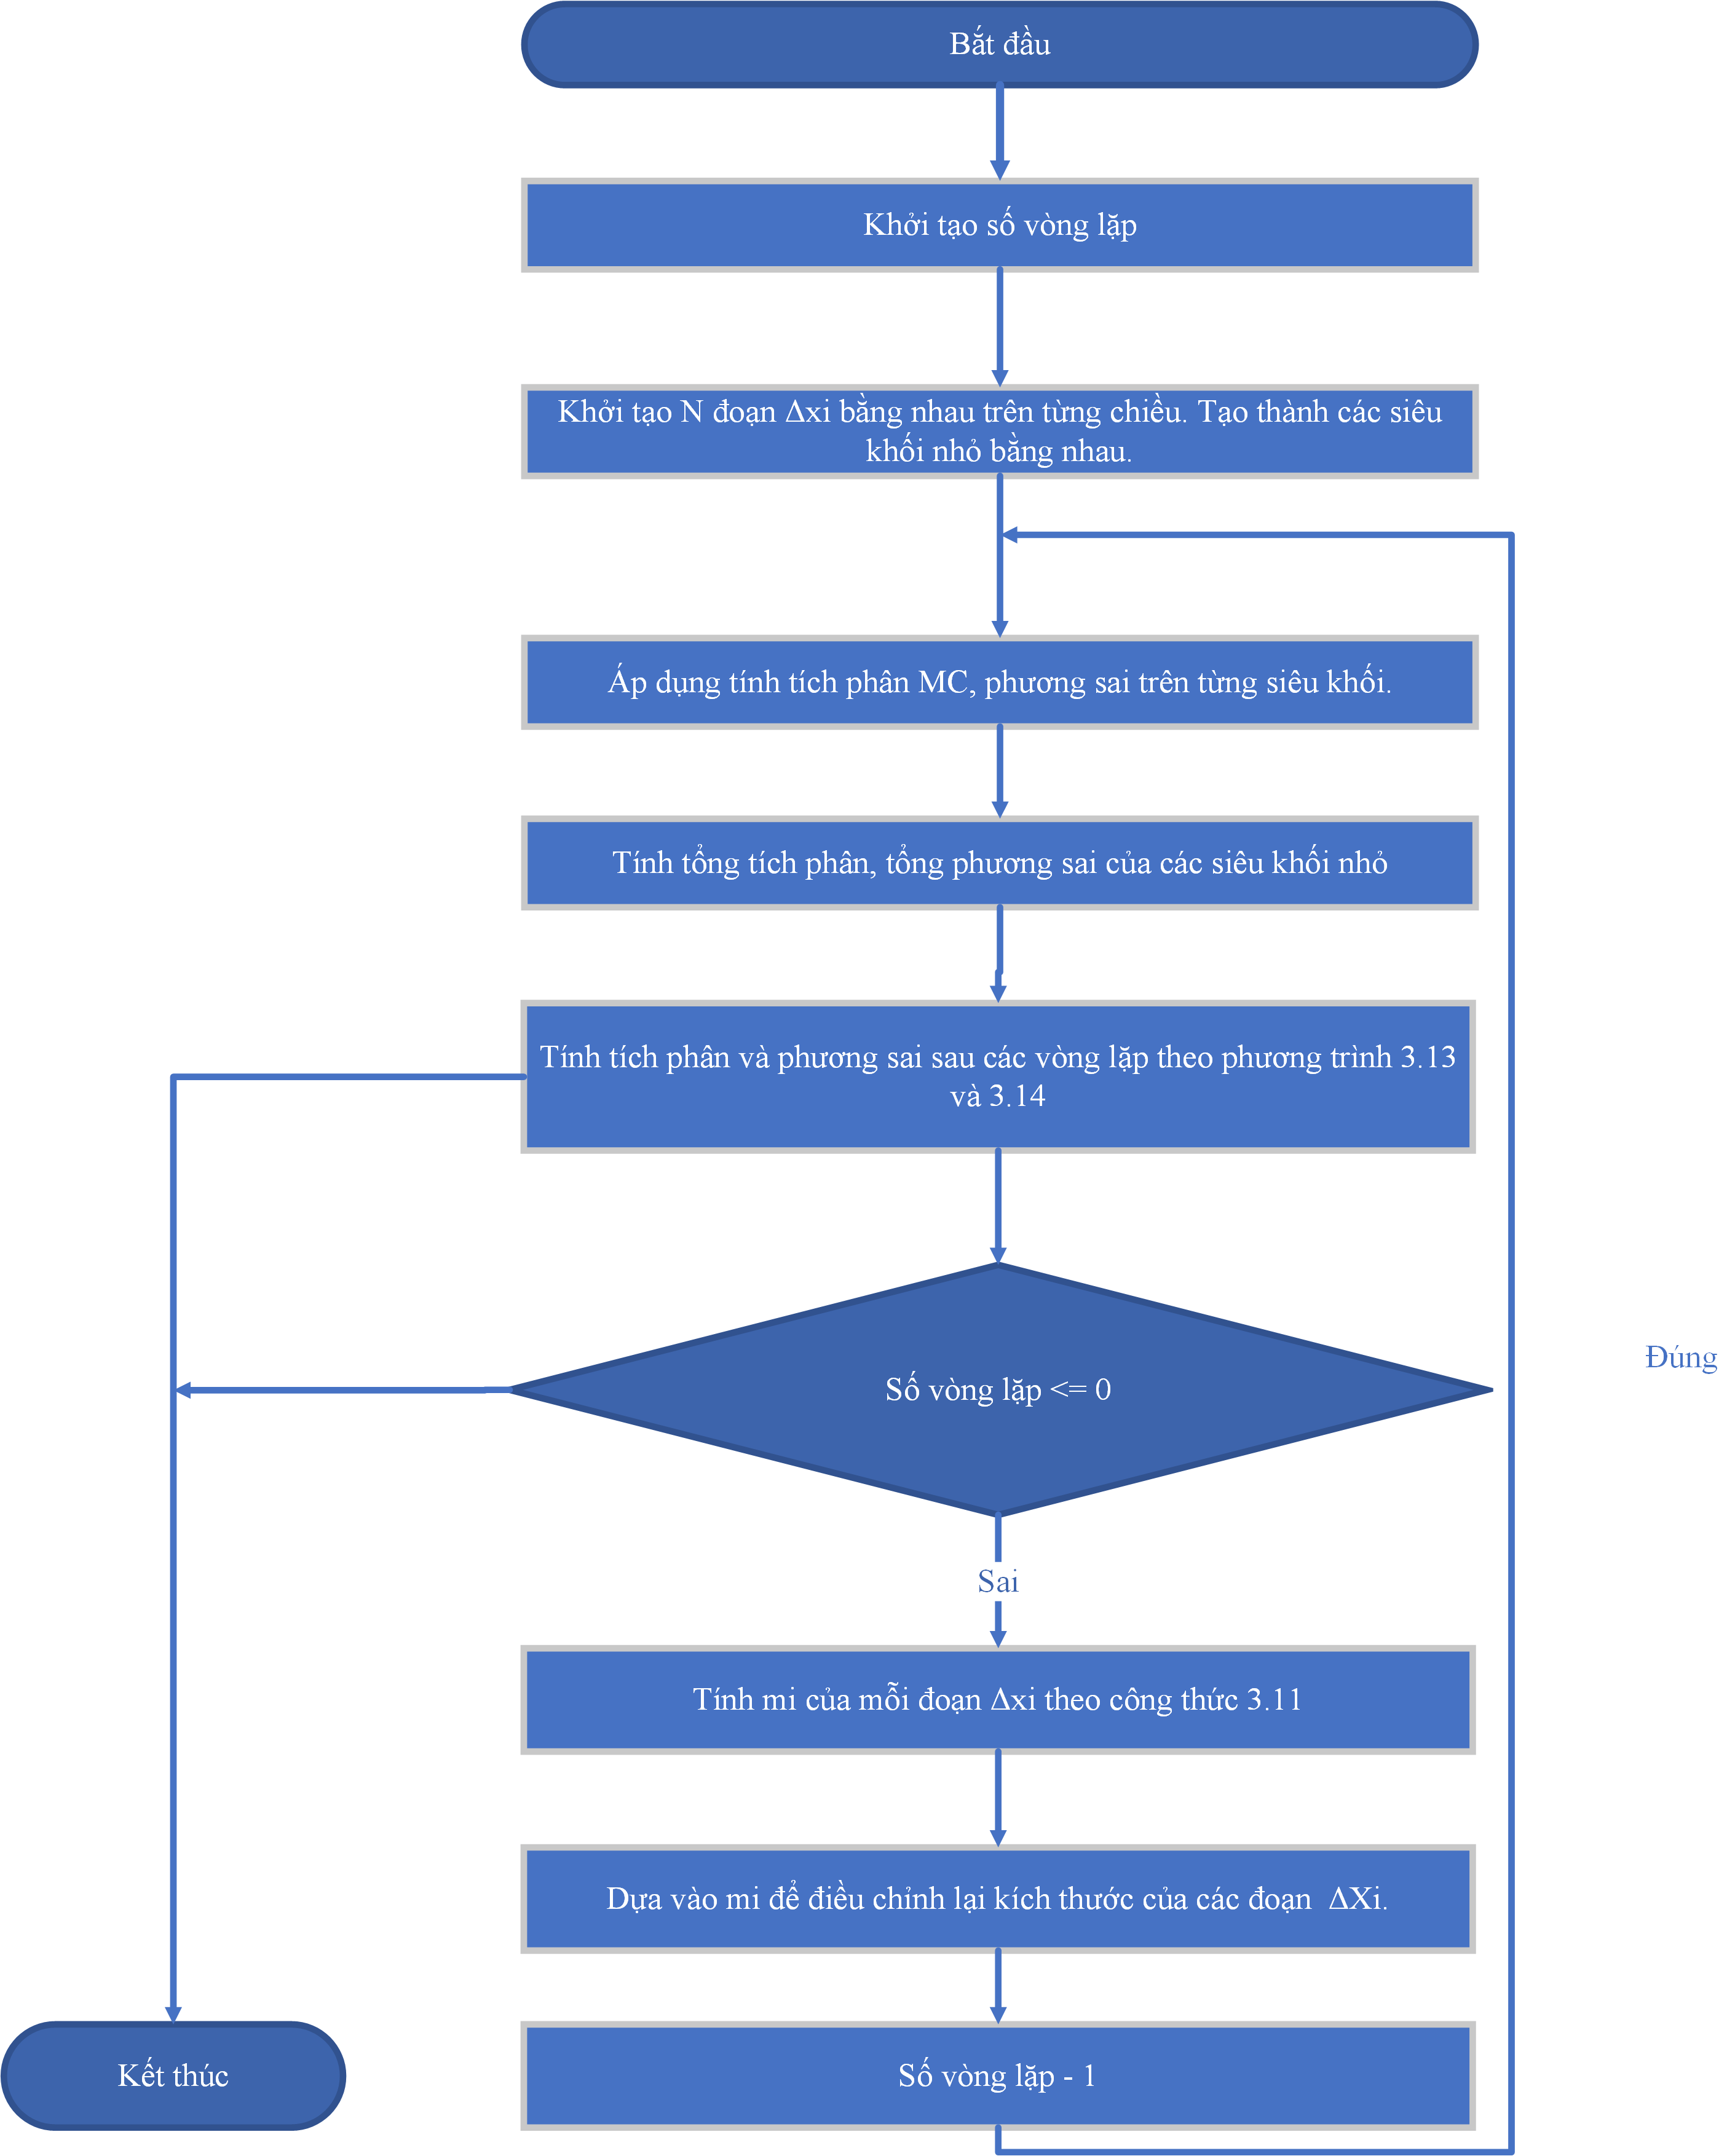
\includegraphics[width=0.95\textwidth]{flowchart_monte.png}
      \caption{Các bước thực hiện thuật toán Vegas}\label{hinh3.1}
\end{figure}
\textbf{Các bước thực hiện }
\begin{itemize}
\item Khởi tạo khối siêu thể tích nhỏ bằng nhau.\par
Giả sử chia đoạn [0,1] thành N đoạn ${\Delta}x_i$. Với $i=0,1, ..., N-1$. 
Sử dụng hàm \textit{rand()} có sẵn trong thư viện của C/C++ để tạo biến ngẫu nhiên đều trong đoạn [0,1].
Xác suất $p(x)$ của biến $x$ trong đoạn ${\Delta}x_i$ bằng $\frac{1}{N{\Delta}x_i}$\\
Xét:
\begin{center}
      $x_0=0$\\
	$x_1=x_0$+${\Delta}x_0$\\
      $x_2=x_1$+${\Delta}x_1$\\
      ...\\
      $x_N=x_{N-1}$+${\Delta}x_{N-1}$=$1$\\
\end{center}
	
Sau đó gán $rc$ = $x_i$ thì giá trị của $rc$ dao động từ 0 đến 1, vậy biến x ngẫu nhiên trên đoạn $[a,b]$ có xác suất $p(x)$ bằng
\begin{align}
	x=a+rc(b-a)
\end{align}
Theo cách giải thích trên, để tạo số ngẫu nhiên đa chiều $\textbf{x}(x_1, x_2, x_3, ..., x_n)$. Xác suất $p(\textbf{x})$ bằng: 
\begin{align}
	p(\textbf{x})=p(x_1)p(x_2)...p(x_n)
\end{align}
Xét tích phân trong miền n chiều, khối siêu thể tích cần được chia thành các siêu khối nhỏ.
Sau đó, tích phân MC sẽ được tính trong các khối nhỏ này. 
Để tạo ra các khối nhỏ bằng nhau, cần chia N đoạn ${\Delta}x_i$ bằng nhau theo mỗi chiều.
% \begin{figure}[H]
%       \centering
%       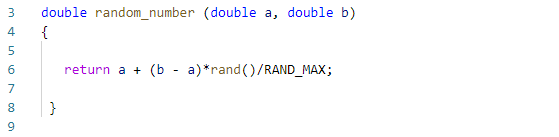
\includegraphics[width=0.99\textwidth]{C_random_number.png}
%       \caption{Hàm rand() tạo biến ngẫu nhiên trong C/C++}\label{hinh3.3.1}
% \end{figure}
% \begin{figure}[H]
%       \centering
%       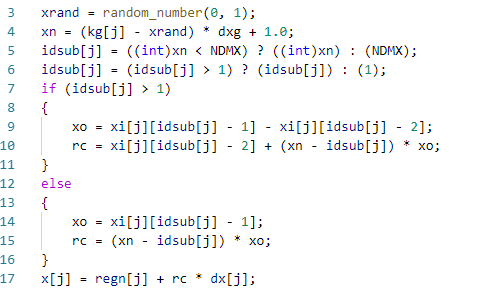
\includegraphics[width=0.95\textwidth]{random_number.png}
%       \caption{Đoạn mã tạo số ngẫu nhiên X theo từng khối nhỏ}\label{hinh3.3}
% \end{figure}
% \item Tạo lưới với các ô có kích thước bằng nhau.\par
% Ban đầu trên mỗi chiều chia thành các đoạn ${\Delta}x_i$ bằng nhau. Sau đó kết hợp lại sẽ thành một lưới như hình $\ref{hinh3.4}$ với hai chiều.
% Hàm \textit{rebin} bên dưới có chức năng tạo thành các đoạn ${\Delta}x_i$ bằng nhau trên mỗi chiều.
% \begin{figure}[H]
%       \centering
%       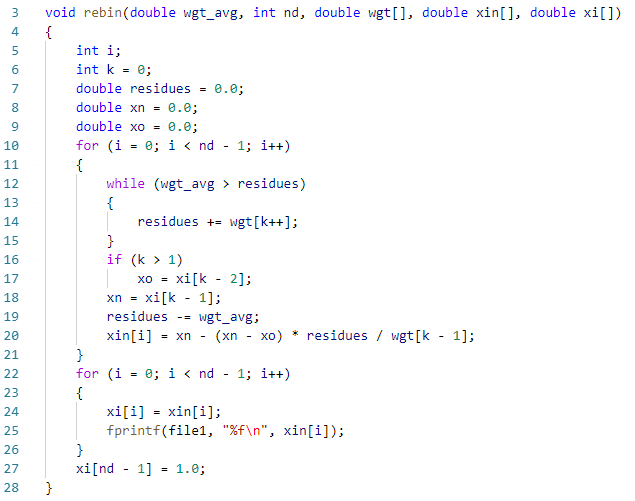
\includegraphics[width=0.99\textwidth]{rebin.png}
%       \caption{Hàm rebin có chức năng điều chỉnh kích thước các đoạn ${\Delta}x_i$}
% \end{figure}
% \begin{figure}[H]
%       \centering
%       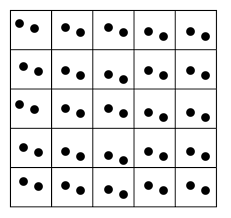
\includegraphics[width=0.6\textwidth]{luoi.png}
%       \caption{Lưới được chia thành các ô bằng nhau}\label{hinh3.4}
% \end{figure}
\item Uớc tính tích phân của từng khối siêu thể tích nhỏ với trọng số wgt.\par
Như vậy ta sử dụng các đoạn [0,1] và ban đầu chia đoạn này thành N đoạn nhỏ ${\Delta}x_i$ bằng nhau. Với $i=0,1, ..., N-1$. 
Với công thức $M=2N^n$. Khởi tạo số mẫu M dùng để tính tích phân, số chiều n. Số điểm ngẫu nhiên cho mỗi khối bằng 2. Suy ra số lượng các khối siêu thể tích nhỏ.
Khởi tạo các miền xác định của từng chiều của biến ngẫu nhiên $x(x_1, x_2, x_3, ..., x_n)$. Mỗi biến giá trị $x_1$, $x_2$, $x_3$,... 
đều được tạo ra thông qua việc lấy ngẫu nhiên từ các đoạn nhỏ ${\Delta}x_i$ từ đoạn [0,1]. Như vậy ban đầu ${\Delta}x_i$ đều bằng nhau thì mật độ các điểm lấy ngẫu nhiên trên miền xác định đều như nhau.
Khi đã tạo được biến ngẫu nhiên \textbf{x} với xác suất p(\textbf{x}) bên trong mỗi khối siêu thể tích nhỏ thì sau cùng tích phân MC bên trong mỗi khối siêu thể tích nhỏ sẽ được tính với trọng số wgt theo công thức sau
            \begin{align}
                  I={\frac{1}{M}}{{\frac{f(\textbf{x})}{p(\textbf{x})}}}\label{pt3.20}
            \end{align}
Sơ đồ khối trong hình $ \ref{hypercube} $ mô tả các bước tính I tại \textbf{x}.
\newline
            \begin{figure}[H]
                        \centering
                        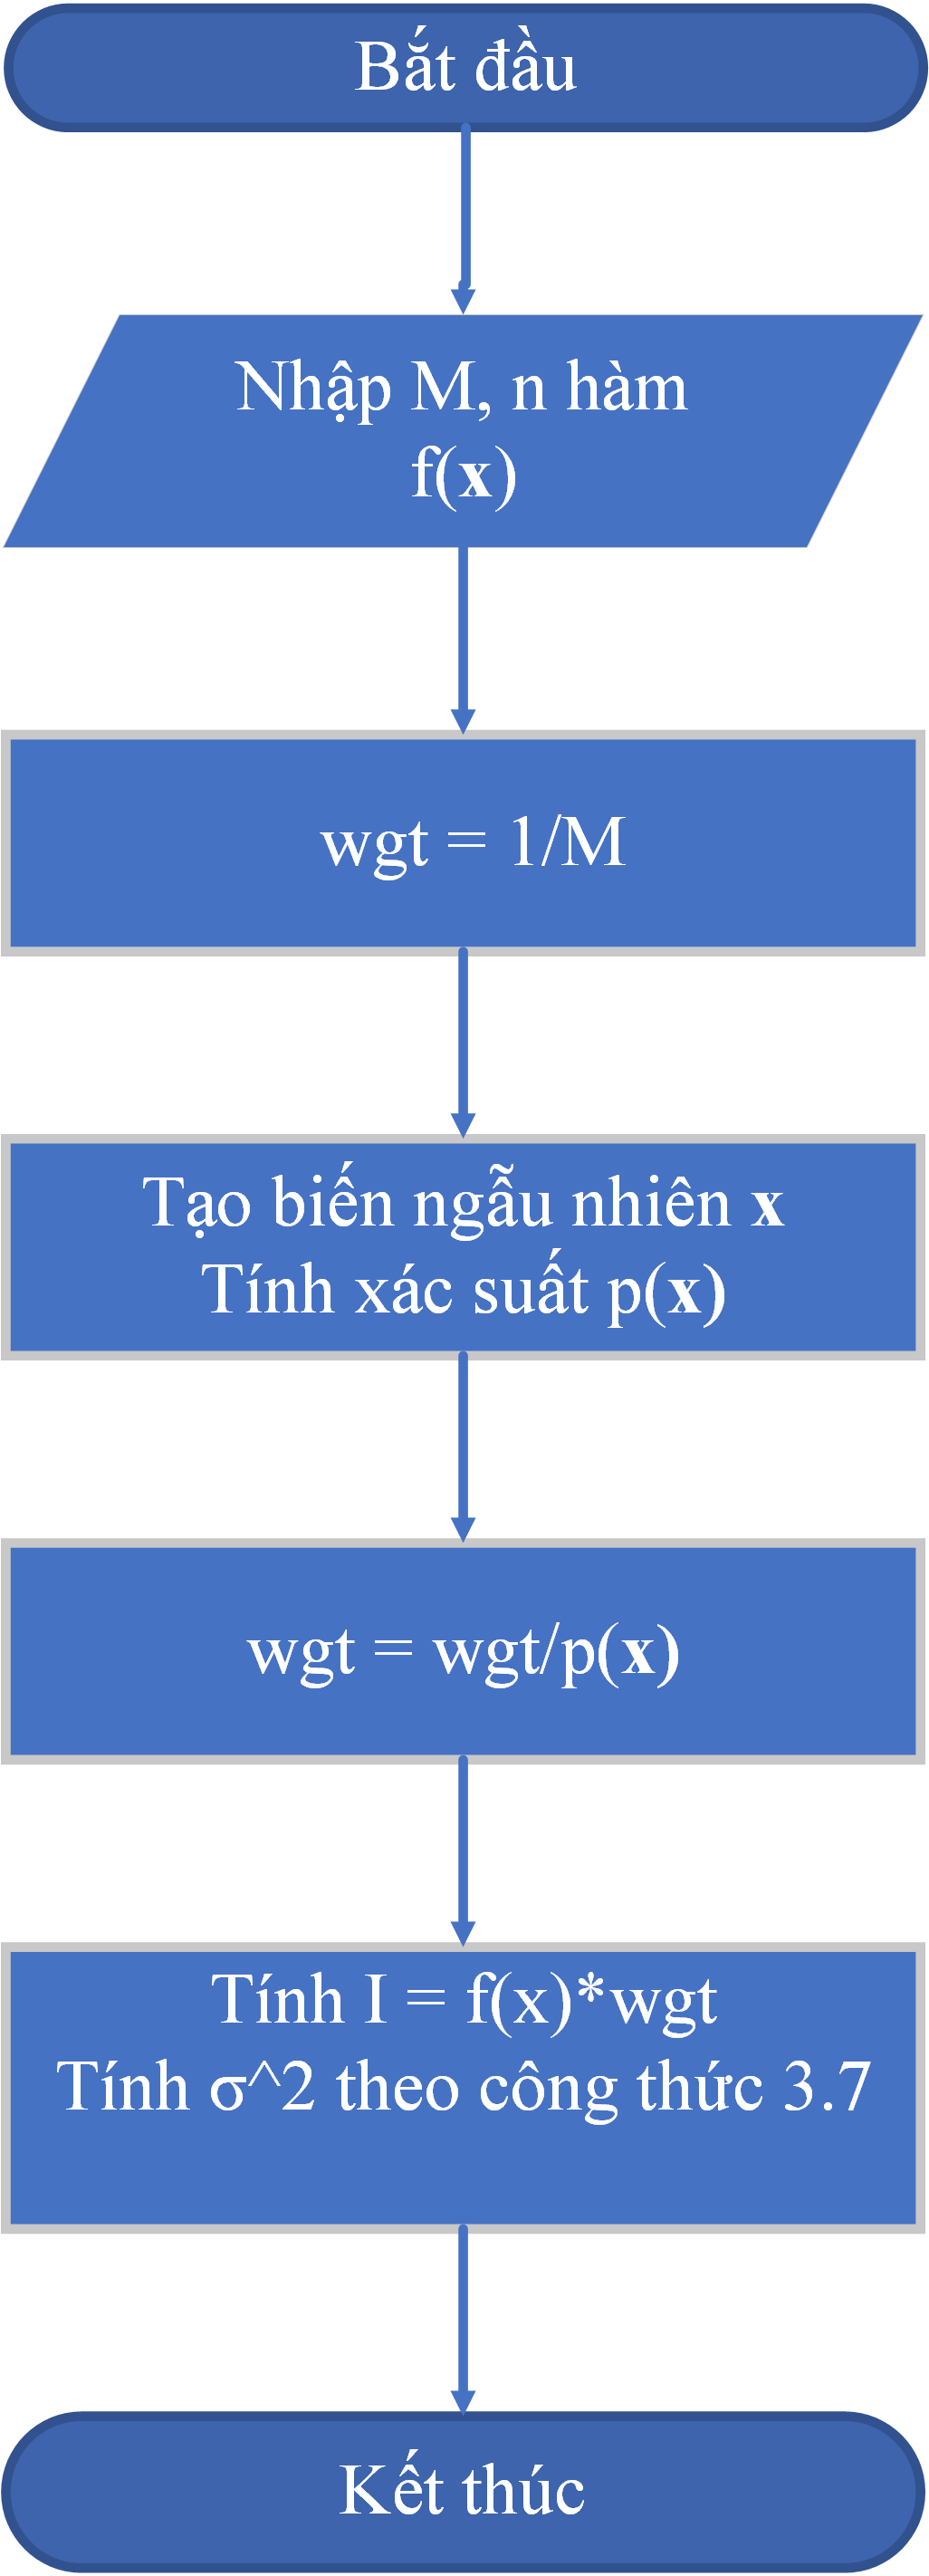
\includegraphics[width=0.36\textwidth]{hypercube.png}
                        \caption{Tích phân bên trong khối siêu thể tích }\label{hypercube}
            \end{figure}
\item Sau khi đã tính các khối tích phân nhỏ thì dễ dàng tính được tổng tích phân của nó dựa vào các thông tin tích phân và phương sai của vòng lặp trước để tính giá trị $m_i$ trong phương trình $\ref{ptmi}$\par
Sơ đồ khối trong hình $ \ref{mi} $ thể hiện thuật toán ước tính tổng tích phân của các đoạn ${\Delta}x_i$.
\begin{figure}[H]
      \centering
      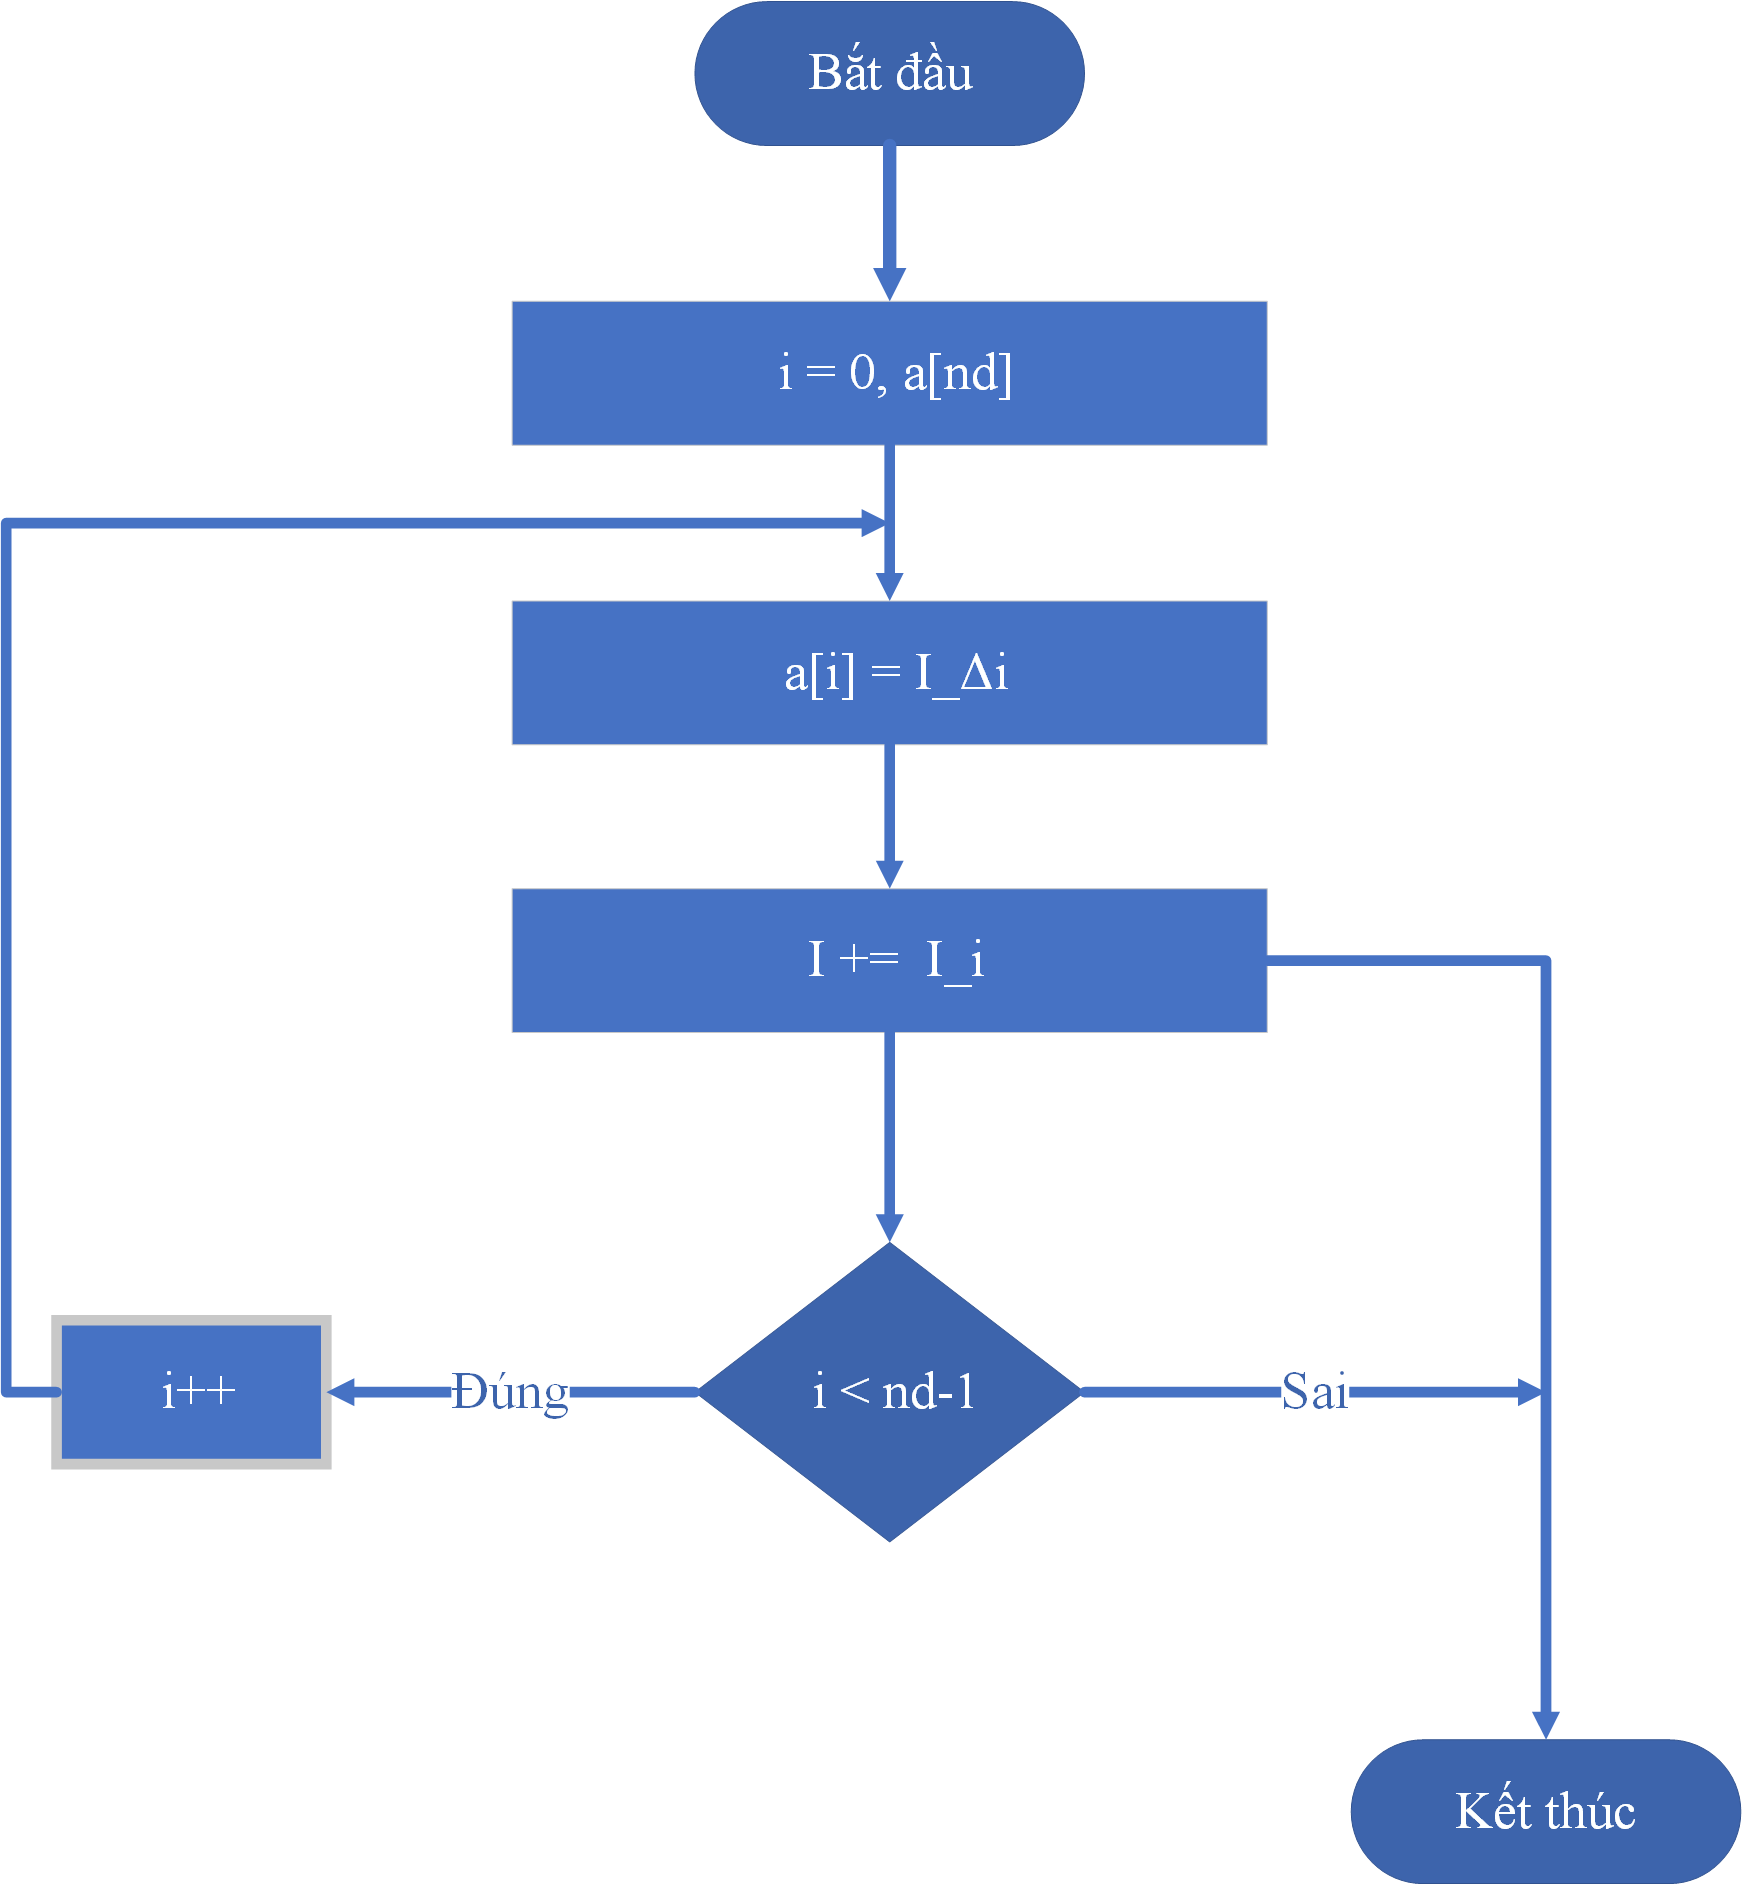
\includegraphics[width=0.85\textwidth]{mi.png}
      \caption{Tính tổng tích phân trên các đoạn ${\Delta}x_i$}\label{mi}
\end{figure}
Trong đó: 
\begin{itemize}
      \item i=1, 0, ..., nd (nd là số đoạn ${\Delta}x_i$)
      \item Mảng a[nd] để lưu giá trị ước tính tích phân trên mỗi đoạn ${\Delta}x_i$.
      \item I là tổng ước tính tích phân của các đoạn ${\Delta}x_i$.
\end{itemize}
Như vậy các giá trị $m_i$ được tính như sau
\begin{center}
      $m_i=I_{\Delta}x_i/I_j$
\end{center}
trong đó $I_j$ là tổng tích phân thuộc vòng lặp trước đó.
Thấy rằng giá trị $m_i$ sau khi tính toán nó thể hiện cho tỉ lệ kích thước mà đoạn ${\Delta}x_i$ có được trên tổng kích thước các đoạn ${\Delta}x_i$.
như được trình bày ở phần $ \ref{giaithichmi} $. Sau đó lấy các giá trị $m_i$ để điều chỉnh lại các đoạn ${\Delta}x_i$.
Với thuật toán Vegas, kích thướt các đoạn ${\Delta}x_i$ sẽ được điều chỉnh theo từng chiều. Kết quả kích thước các khối siêu thể tích sẽ được điều chỉnh.
Hay nói cách khác, mật độ điểm gieo sẽ tập trung tại nhưng nơi có tích phân lớn. Từ đó giảm sai số cho ước tính tích phân.

\item Ước tổng tính tích phân và độ lệch chuẩn qua các vòng lặp.\par
Khi đã có giá trị tích phân f(x) tại x và phương sai $\sigma^2$ bên trong từng khối siêu thể tích nhỏ.
Sau đó ước tính giá trị tích phân và độ lệch chuẩn trong từng vòng lặp.  \par
Sơ đồ khối trong hình $ \ref{loops} $ thể hiện thuật toán ước tính tích phân và độ lệch chuẩn qua các vòng lặp.
\begin{figure}[H]
      \centering
      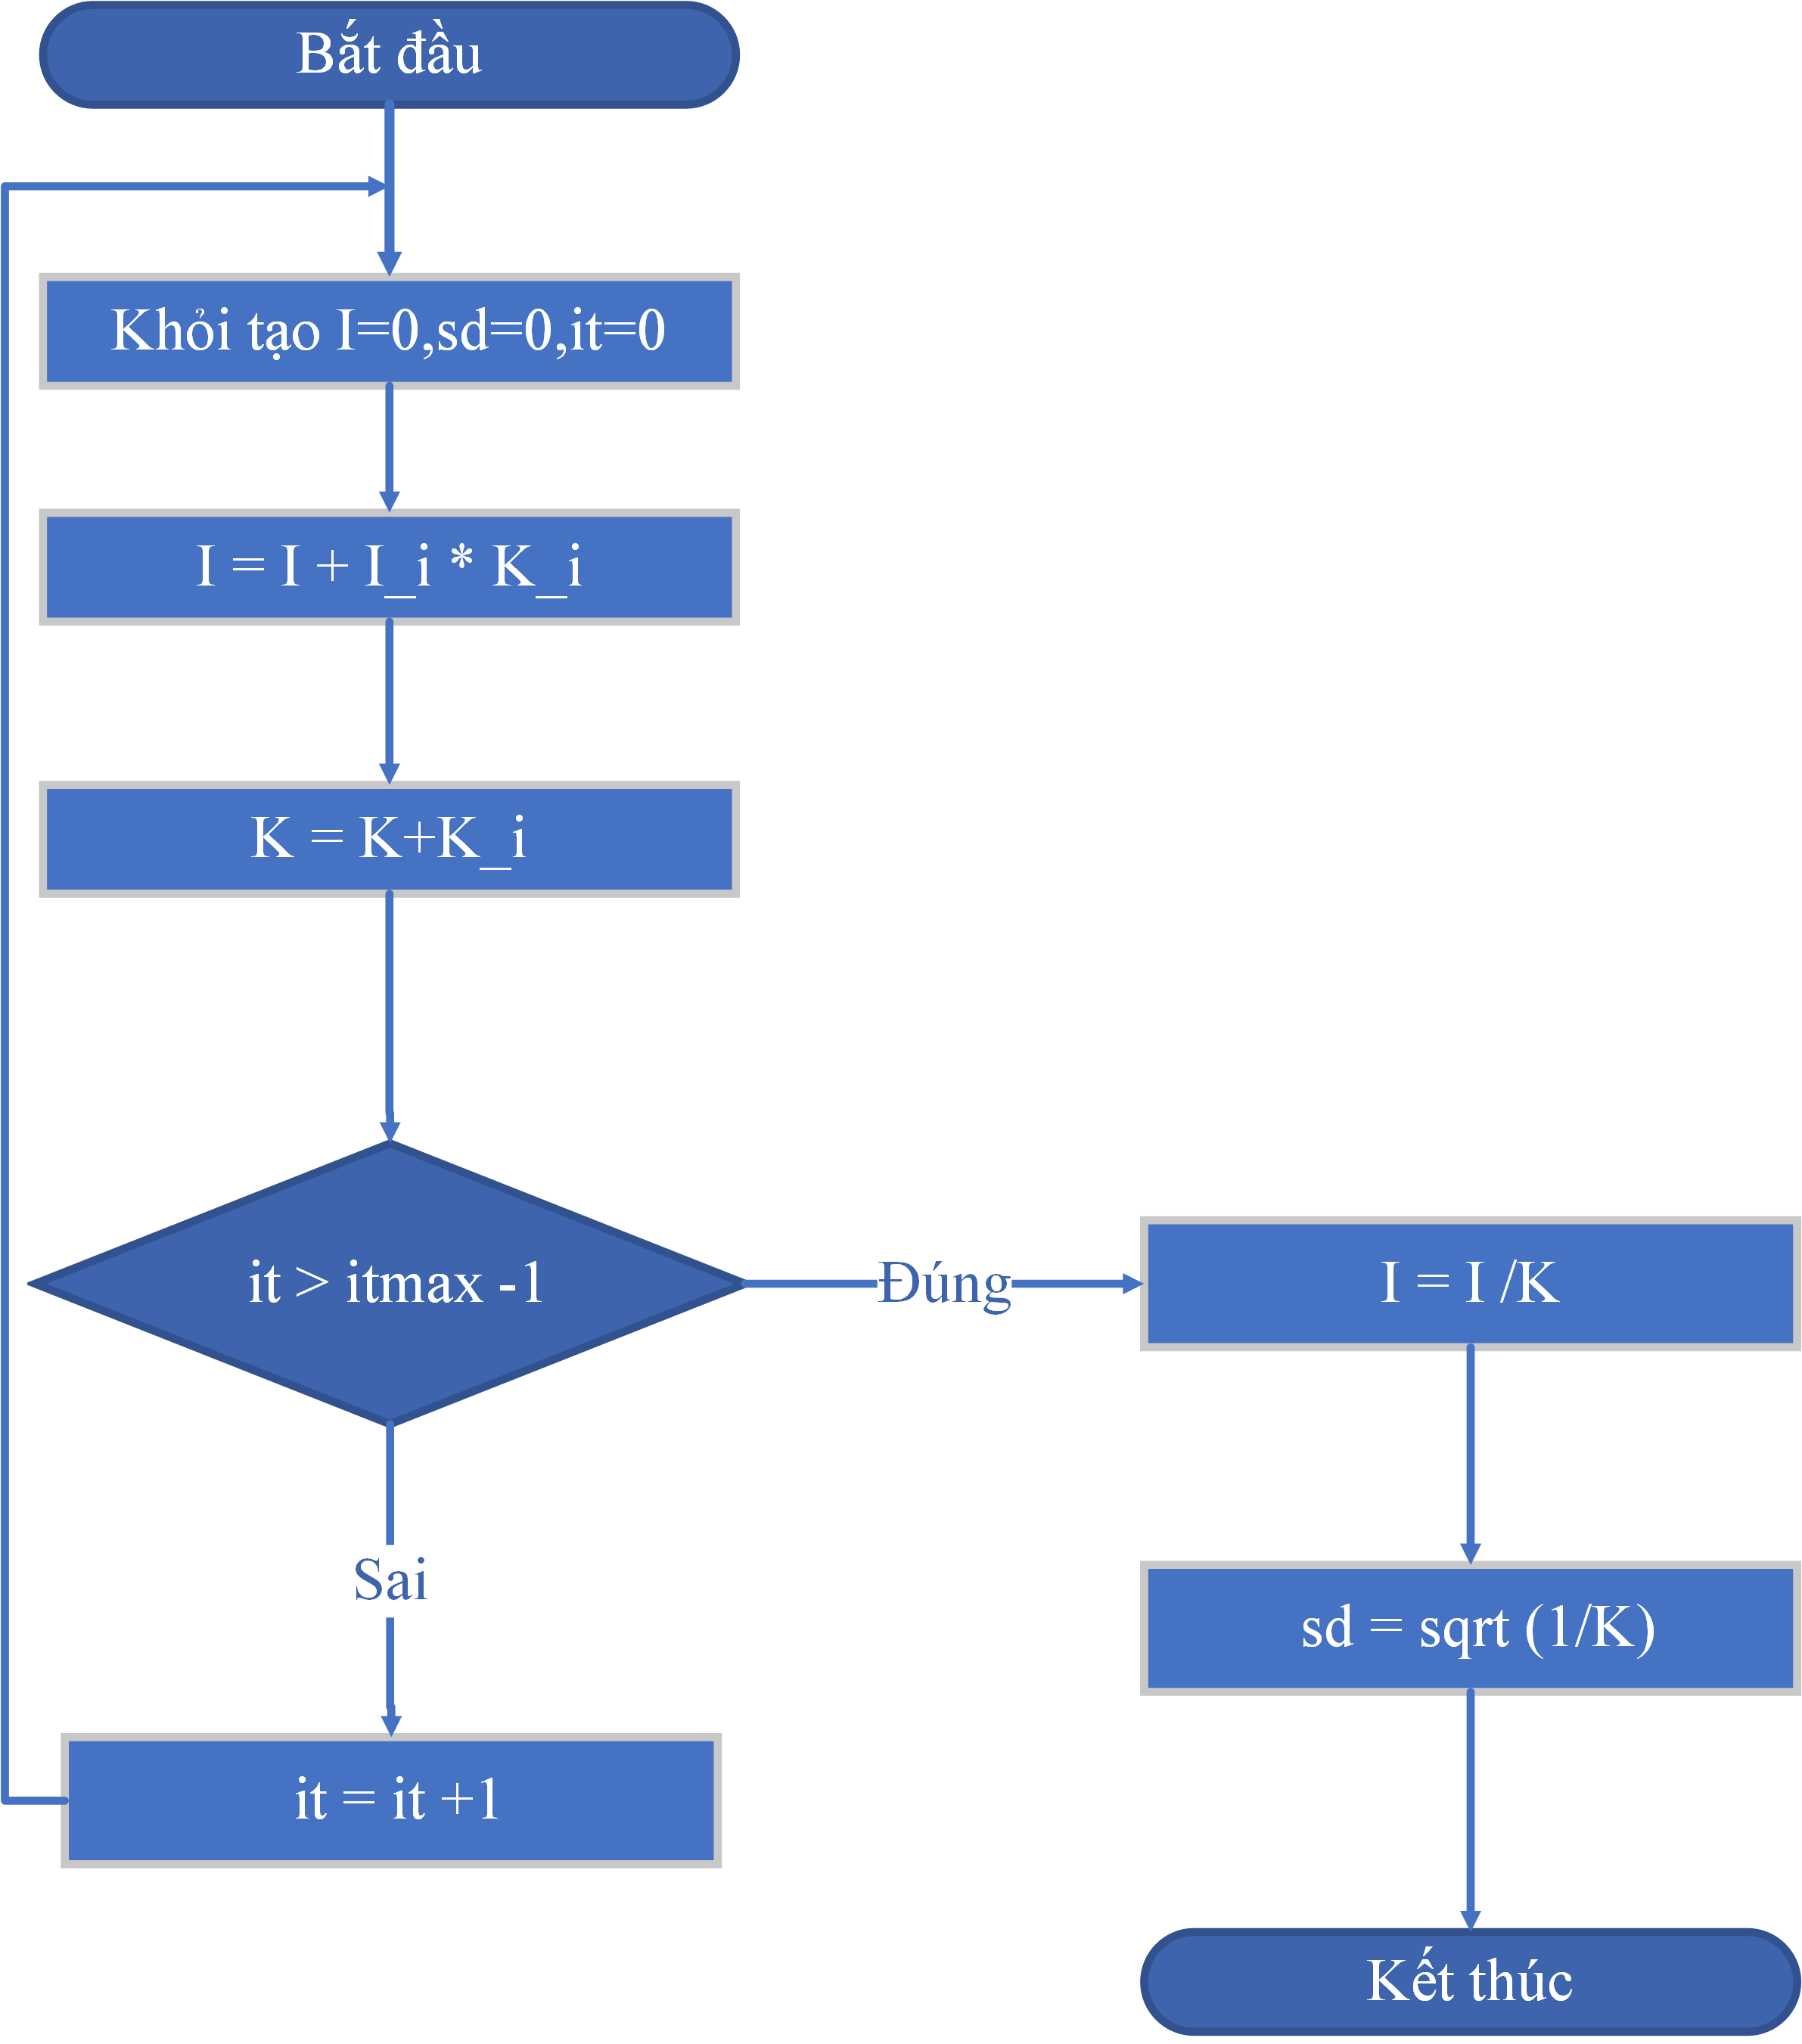
\includegraphics[width=0.85\textwidth]{loops.png}
      \caption{Tính giá trị hàm f(x) tại x với trọng số }\label{loops}
\end{figure}
Trong đó
\begin{itemize}
      \item it là biến đếm vòng lặp.
      \item itmax là số vòng lặp.
      \item I là ước tính tích phân khi kết thúc vòng lặp.
      \item $I_i$ là Ước tính tích phân qua các vòng lặp.
\end{itemize}
Khi kết thúc vòng lặp đây sẽ là kết quả ước tính tích phân và sai số cuối cùng của hàm $f(x)$.
\end{itemize}



